\section{Results}
\label{sec:results}
In this section we describe the results obtained from our simulations.
The section is devided into two parts. The first part presents the
constants we use and the scenarios that we simulate and comment on
the general success of our implementation of the model. We looked
for unrealistic or unexpected behavior in our simulations. In the
last part we present the results from our attempts to replicate
the phenomena presented in \cite{self-org}.Possible remedies for
any discrepancies between the expected and the actual results are
discussed in section~\ref{sec:discussion}.

\subsection{The basics}
This section is devided into three parts. First we present the
scenarios that we have simulated, then we present the constants
used in the simulations. We then move on to comment on the
general behavior of the pedestrians in our simulations.

\subsubsection{Scenarios}
We simulate four different scenarios, a rectangle shaped room with a
door in the middle of one of the walls, and three different variations
of corridors; a normal corridor, a corridor with a bottleneck in the
middle and a corridor with a sudden open space. In the corridors we have
the opportunity to make bidirectional flow. Screen shots from each
scenario are presented in figure \ref{fig:fourcases}.

\begin{figure}[h]
\centering
\subfloat[Square room.]{\resizebox{4cm}{!}{\begin{tikzpicture}

\end{tikzpicture}
}}
\subfloat[Bottleneck.]{\resizebox{7cm}{!}{\begin{tikzpicture}
\draw[color=blue] (10.20,-0.82) circle (0.21);
\draw[color=blue] (11.02,-1.97) circle (0.20);
\draw[color=blue] (9.63,-0.94) circle (0.20);
\draw[color=blue] (11.62,-0.29) circle (0.19);
\draw[color=blue] (11.47,2.10) circle (0.18);
\draw[color=blue] (10.48,-2.41) circle (0.19);
\draw[color=blue] (5.77,0.15) circle (0.20);
\draw[color=blue] (9.33,1.17) circle (0.20);
\draw[color=blue] (11.70,0.48) circle (0.20);
\draw[color=blue] (10.58,-0.16) circle (0.20);
\draw[color=blue] (10.44,1.08) circle (0.19);
\draw[color=blue] (12.15,1.00) circle (0.18);
\draw[color=blue] (11.04,1.59) circle (0.19);
\draw[color=blue] (9.23,-0.44) circle (0.19);
\draw[color=blue] (6.84,-1.70) circle (0.20);
\draw[color=blue] (8.87,1.83) circle (0.20);
\draw[color=blue] (6.54,-0.44) circle (0.18);
\draw[color=blue] (10.86,-1.36) circle (0.21);
\draw[color=blue] (9.88,0.21) circle (0.20);
\draw[color=blue] (9.89,-1.87) circle (0.20);
\draw[color=blue] (6.04,-1.63) circle (0.21);
\draw[color=blue] (8.87,0.53) circle (0.21);
\draw[color=blue] (7.99,0.26) circle (0.20);
\draw[color=blue] (5.41,-0.25) circle (0.20);
\draw[color=blue] (11.07,0.44) circle (0.20);
\draw[color=blue] (8.60,-0.27) circle (0.20);
\draw[color=blue] (7.87,1.96) circle (0.19);
\draw[color=blue] (7.11,0.68) circle (0.20);
\draw[color=blue] (8.43,1.00) circle (0.20);
\draw[color=blue] (7.83,-0.50) circle (0.19);
\draw[color=blue] (8.64,-1.20) circle (0.21);
\draw[color=blue] (9.34,-1.40) circle (0.20);
\draw[color=blue] (4.83,-0.64) circle (0.21);
\draw[color=blue] (6.07,-0.86) circle (0.19);
\draw[color=blue] (6.45,0.89) circle (0.21);
\draw[color=blue] (7.89,1.19) circle (0.19);
\draw[color=blue] (1.67,-0.57) circle (0.20);
\draw[color=blue] (6.05,1.61) circle (0.20);
\draw[color=blue] (5.49,-1.13) circle (0.20);
\draw[color=blue] (4.13,0.72) circle (0.20);
\draw[color=blue] (3.48,-0.13) circle (0.20);
\draw[color=blue] (3.54,0.51) circle (0.19);
\draw[color=blue] (4.60,-1.25) circle (0.20);
\draw[color=blue] (3.76,-1.28) circle (0.20);
\draw[color=blue] (5.80,0.82) circle (0.20);
\draw[color=blue] (5.09,0.53) circle (0.18);
\draw[color=blue] (0.27,-0.23) circle (0.19);
\draw[color=blue] (2.15,-0.14) circle (0.18);
\draw[color=blue] (4.12,-0.39) circle (0.20);
\draw[color=blue] (5.03,1.23) circle (0.19);
\draw[color=blue] (2.85,0.76) circle (0.21);
\draw[color=blue] (3.49,1.13) circle (0.19);
\draw[color=blue] (3.39,-0.85) circle (0.21);
\draw[color=blue] (-2.42,-1.28) circle (0.19);
\draw[color=blue] (0.41,0.15) circle (0.22);
\draw[color=blue] (4.91,0.01) circle (0.20);
\draw[color=blue] (2.96,0.05) circle (0.20);
\draw[color=blue] (-1.40,0.87) circle (0.18);
\draw[color=blue] (1.40,-0.17) circle (0.19);
\draw[color=blue] (-0.07,0.31) circle (0.20);
\draw[color=blue] (2.70,-0.66) circle (0.20);
\draw[color=blue] (-0.88,-0.27) circle (0.19);
\draw[color=blue] (1.68,0.44) circle (0.19);
\draw[color=blue] (2.34,0.58) circle (0.20);
\draw[color=blue] (-0.24,-0.22) circle (0.21);
\draw[color=blue] (-0.46,0.41) circle (0.21);
\draw[color=blue] (0.94,-0.05) circle (0.19);
\draw[color=blue] (-0.92,0.14) circle (0.19);
\draw[color=blue] (-0.67,-0.63) circle (0.21);
\draw[color=blue] (-1.38,-0.47) circle (0.19);
\draw[color=blue] (-1.89,0.99) circle (0.21);
\draw[color=blue] (-1.76,0.15) circle (0.20);
\draw[color=blue] (-2.41,1.34) circle (0.20);
\draw[color=blue] (-2.18,-0.65) circle (0.18);
\draw[color=blue] (-0.95,0.61) circle (0.19);
\draw[color=blue] (-1.46,-0.97) circle (0.21);
\draw[color=blue] (-2.67,-0.12) circle (0.19);
\draw[color=blue] (-3.08,-1.51) circle (0.19);
\draw[color=blue] (-4.20,1.96) circle (0.22);
\draw[color=blue] (-3.33,1.39) circle (0.21);
\draw[color=blue] (-3.10,-0.80) circle (0.20);
\draw[color=blue] (-4.15,1.04) circle (0.19);
\draw[color=blue] (-3.71,-1.07) circle (0.22);
\draw[color=blue] (-2.49,0.61) circle (0.19);
\draw[color=blue] (-3.55,-1.91) circle (0.20);
\draw[color=blue] (-3.31,-0.17) circle (0.18);
\draw[color=blue] (-4.55,-0.92) circle (0.21);
\draw[color=blue] (-3.10,0.61) circle (0.20);
\draw[color=blue] (-3.90,0.00) circle (0.20);
\draw[color=blue] (-4.83,1.46) circle (0.21);
\draw[color=blue] (-5.43,0.90) circle (0.20);
\draw[color=blue] (-4.93,-1.33) circle (0.20);
\draw[color=blue] (-4.79,0.18) circle (0.21);
\draw[color=blue] (-5.65,-0.68) circle (0.21);
\draw[color=blue] (-5.97,1.31) circle (0.20);
\draw[color=blue] (-5.56,0.01) circle (0.22);
\draw[color=blue] (-5.76,-1.47) circle (0.20);
\draw[color=blue] (-6.06,0.46) circle (0.19);
\draw[color=blue] (-7.12,1.03) circle (0.20);
\draw[color=blue] (-6.41,-0.92) circle (0.20);
\draw[color=blue] (-7.05,-1.14) circle (0.18);
\draw[color=blue] (-6.56,-0.19) circle (0.21);
\draw[color=blue] (-7.82,-1.02) circle (0.21);
\draw[color=blue] (-7.69,0.99) circle (0.20);
\draw[color=blue] (-7.09,0.32) circle (0.21);
\draw[color=blue] (-7.55,-0.00) circle (0.19);
\draw[color=blue] (-8.21,0.32) circle (0.19);
\draw[color=blue] (-7.85,-0.40) circle (0.19);
\draw[color=blue] (-8.77,0.80) circle (0.19);
\draw[color=blue] (-8.95,-0.09) circle (0.20);
\draw[color=blue] (-9.22,-0.80) circle (0.20);
\draw[color=blue] (-8.59,-0.84) circle (0.21);
\draw[color=blue] (-9.39,0.70) circle (0.20);
\draw[color=blue] (-9.73,0.68) circle (0.21);
%\node at (-12.50, 5.83) {t = 40.26};
\useasboundingbox (-12.50, -5.83) rectangle (12.50, 5.83);
\draw[color=black] (-10.00,3.00) -- (-5.00,3.00);
\draw[color=black] (-10.00,-3.00) -- (-5.00,-3.00);
\draw[color=black] (-5.00,3.00) -- (0.00,0.50);
\draw[color=black] (-5.00,-3.00) -- (0.00,-0.50);
\draw[color=black] (0.00,0.50) -- (5.00,3.00);
\draw[color=black] (0.00,-0.50) -- (5.00,-3.00);
\draw[color=black] (5.00,3.00) -- (10.00,3.00);
\draw[color=black] (5.00,-3.00) -- (10.00,-3.00);
\end{tikzpicture}
}}\\
\subfloat[Corridor.]{\resizebox{7cm}{!}{\begin{tikzpicture}
\draw[color=blue] (11.86,0.21) circle (0.21);
\draw[color=blue] (12.23,-1.26) circle (0.19);
\draw[color=blue] (11.20,0.43) circle (0.21);
\draw[color=blue] (11.84,1.02) circle (0.20);
\draw[color=blue] (12.21,-0.58) circle (0.20);
\draw[color=blue] (10.65,0.54) circle (0.19);
\draw[color=blue] (11.47,-0.42) circle (0.20);
\draw[color=blue] (10.31,-0.21) circle (0.20);
\draw[color=blue] (10.09,0.52) circle (0.20);
\draw[color=blue] (9.67,-0.59) circle (0.21);
\draw[color=blue] (10.79,-0.65) circle (0.19);
\draw[color=blue] (8.99,-0.61) circle (0.17);
\draw[color=blue] (8.40,0.19) circle (0.20);
\draw[color=blue] (8.02,-0.08) circle (0.19);
\draw[color=blue] (9.02,-0.04) circle (0.18);
\draw[color=blue] (9.53,0.55) circle (0.19);
\draw[color=blue] (9.70,-0.02) circle (0.21);
\draw[color=blue] (8.54,-0.52) circle (0.20);
\draw[color=blue] (7.38,-0.12) circle (0.20);
\draw[color=blue] (7.99,-0.62) circle (0.20);
\draw[color=blue] (9.05,0.58) circle (0.19);
\draw[color=blue] (7.12,-0.63) circle (0.21);
\draw[color=blue] (6.73,-0.23) circle (0.20);
\draw[color=blue] (6.29,-0.68) circle (0.21);
\draw[color=blue] (6.99,0.51) circle (0.20);
\draw[color=blue] (5.63,-0.56) circle (0.20);
\draw[color=blue] (6.39,0.67) circle (0.21);
\draw[color=blue] (5.90,0.69) circle (0.20);
\draw[color=blue] (5.26,-0.79) circle (0.19);
\draw[color=blue] (6.07,-0.20) circle (0.21);
\draw[color=blue] (5.24,0.63) circle (0.20);
\draw[color=blue] (6.51,0.18) circle (0.19);
\draw[color=blue] (5.72,0.30) circle (0.21);
\draw[color=blue] (8.44,0.68) circle (0.19);
\draw[color=blue] (2.95,-0.67) circle (0.19);
\draw[color=blue] (4.81,-0.04) circle (0.23);
\draw[color=blue] (4.80,0.54) circle (0.19);
\draw[color=blue] (4.50,-0.67) circle (0.20);
\draw[color=blue] (7.76,0.48) circle (0.19);
\draw[color=blue] (3.48,0.17) circle (0.19);
\draw[color=blue] (5.48,-0.06) circle (0.21);
\draw[color=blue] (2.24,-0.57) circle (0.19);
\draw[color=blue] (1.65,-0.50) circle (0.21);
\draw[color=blue] (4.42,0.69) circle (0.19);
\draw[color=blue] (3.85,0.57) circle (0.20);
\draw[color=blue] (3.64,-0.48) circle (0.20);
\draw[color=blue] (4.38,0.16) circle (0.19);
\draw[color=blue] (3.29,0.72) circle (0.21);
\draw[color=blue] (5.10,-0.43) circle (0.20);
\draw[color=blue] (2.35,0.58) circle (0.20);
\draw[color=blue] (4.16,-0.31) circle (0.20);
\draw[color=blue] (1.83,0.41) circle (0.22);
\draw[color=blue] (0.60,0.09) circle (0.20);
\draw[color=blue] (0.58,0.63) circle (0.20);
\draw[color=blue] (2.99,0.36) circle (0.19);
\draw[color=blue] (1.14,0.55) circle (0.19);
\draw[color=blue] (2.57,-0.05) circle (0.20);
\draw[color=blue] (3.26,-0.22) circle (0.20);
\draw[color=blue] (1.18,-0.57) circle (0.20);
\draw[color=blue] (1.51,0.01) circle (0.20);
\draw[color=blue] (0.65,-0.60) circle (0.21);
\draw[color=blue] (0.26,-0.23) circle (0.19);
\draw[color=blue] (-0.31,0.02) circle (0.21);
\draw[color=blue] (-0.07,-0.61) circle (0.21);
\draw[color=blue] (-1.00,0.09) circle (0.21);
\draw[color=blue] (-1.75,-0.08) circle (0.22);
\draw[color=blue] (0.12,0.55) circle (0.20);
\draw[color=blue] (-0.42,0.60) circle (0.20);
\draw[color=blue] (-0.61,-0.66) circle (0.20);
\draw[color=blue] (-0.94,-0.42) circle (0.20);
\draw[color=blue] (-1.60,0.52) circle (0.21);
\draw[color=blue] (-1.55,-0.61) circle (0.19);
\draw[color=blue] (-0.98,0.62) circle (0.20);
\draw[color=blue] (-2.45,-0.06) circle (0.22);
\draw[color=blue] (-2.47,-0.62) circle (0.20);
\draw[color=blue] (-2.98,-0.47) circle (0.20);
\draw[color=blue] (-2.28,0.60) circle (0.20);
\draw[color=blue] (-2.73,0.44) circle (0.20);
\draw[color=blue] (-3.28,0.62) circle (0.19);
\draw[color=blue] (-3.42,-0.63) circle (0.20);
\draw[color=blue] (-3.33,0.00) circle (0.21);
\draw[color=blue] (-3.78,0.22) circle (0.20);
\draw[color=blue] (-4.13,0.63) circle (0.19);
\draw[color=blue] (-3.93,-0.47) circle (0.20);
\draw[color=blue] (-4.51,-0.59) circle (0.20);
\draw[color=blue] (-4.37,0.04) circle (0.19);
\draw[color=blue] (-4.83,0.05) circle (0.21);
\draw[color=blue] (-4.82,0.62) circle (0.20);
\draw[color=blue] (-5.52,0.56) circle (0.20);
\draw[color=blue] (-6.21,0.15) circle (0.21);
\draw[color=blue] (-5.77,-0.52) circle (0.20);
\draw[color=blue] (-5.02,-0.58) circle (0.19);
\draw[color=blue] (-5.36,-0.03) circle (0.20);
\draw[color=blue] (-6.42,-0.52) circle (0.19);
\draw[color=blue] (-7.00,-0.42) circle (0.20);
\draw[color=blue] (-6.46,0.67) circle (0.20);
\draw[color=blue] (-6.70,0.17) circle (0.21);
\draw[color=blue] (-7.57,-0.63) circle (0.20);
\draw[color=blue] (-7.49,-0.04) circle (0.22);
\draw[color=blue] (-7.99,0.07) circle (0.19);
\draw[color=blue] (-8.08,-0.58) circle (0.21);
\draw[color=blue] (-7.43,0.56) circle (0.19);
\draw[color=blue] (-8.40,0.54) circle (0.20);
\draw[color=blue] (-7.90,0.71) circle (0.21);
\draw[color=blue] (-8.61,-0.83) circle (0.21);
\draw[color=blue] (-8.52,-0.15) circle (0.20);
\draw[color=blue] (-8.75,0.38) circle (0.22);
\draw[color=blue] (-8.81,-0.37) circle (0.21);
\draw[color=blue] (-9.17,-0.13) circle (0.21);
\draw[color=blue] (-9.71,-0.45) circle (0.20);
%\node at (-12.50, 5.83) {t = 52.31};
\useasboundingbox (-12.50, -5.83) rectangle (12.50, 5.83);
\draw[color=black] (-10.00,1.00) -- (10.00,1.00);
\draw[color=black] (-10.00,-1.00) -- (10.00,-1.00);
\end{tikzpicture}
}}
\subfloat[Corridor with an opening.]{\resizebox{7cm}{!}{\begin{tikzpicture}
\draw[color=blue] (11.31,-0.03) circle (0.19);
\draw[color=blue] (10.64,0.09) circle (0.21);
\draw[color=blue] (11.61,-1.36) circle (0.20);
\draw[color=blue] (12.40,0.11) circle (0.19);
\draw[color=blue] (11.30,-0.94) circle (0.19);
\draw[color=blue] (2.40,-0.58) circle (0.20);
\draw[color=blue] (11.08,-0.47) circle (0.22);
\draw[color=blue] (9.19,0.66) circle (0.19);
\draw[color=blue] (11.94,1.38) circle (0.19);
\draw[color=blue] (10.63,-1.16) circle (0.19);
\draw[color=blue] (10.27,0.33) circle (0.20);
\draw[color=blue] (11.32,1.21) circle (0.19);
\draw[color=blue] (8.40,-0.12) circle (0.21);
\draw[color=blue] (7.53,-0.58) circle (0.21);
\draw[color=blue] (10.05,0.76) circle (0.21);
\draw[color=blue] (5.65,0.02) circle (0.19);
\draw[color=blue] (10.55,-0.39) circle (0.20);
\draw[color=blue] (11.42,0.53) circle (0.20);
\draw[color=blue] (12.45,-0.53) circle (0.21);
\draw[color=blue] (4.83,-0.17) circle (0.19);
\draw[color=blue] (8.34,-0.64) circle (0.21);
\draw[color=blue] (7.09,-0.65) circle (0.19);
\draw[color=blue] (8.42,0.35) circle (0.18);
\draw[color=blue] (12.18,0.62) circle (0.20);
\draw[color=blue] (8.93,0.34) circle (0.21);
\draw[color=blue] (10.81,0.85) circle (0.21);
\draw[color=blue] (10.01,-0.19) circle (0.20);
\draw[color=blue] (7.91,-0.19) circle (0.20);
\draw[color=blue] (4.92,-0.57) circle (0.20);
\draw[color=blue] (4.82,0.74) circle (0.20);
\draw[color=blue] (7.64,0.24) circle (0.21);
\draw[color=blue] (9.81,0.37) circle (0.20);
\draw[color=blue] (2.98,1.07) circle (0.21);
\draw[color=blue] (10.34,-0.78) circle (0.20);
\draw[color=blue] (9.48,-0.01) circle (0.18);
\draw[color=blue] (3.91,0.68) circle (0.18);
\draw[color=blue] (1.40,-0.42) circle (0.20);
\draw[color=blue] (1.99,-0.25) circle (0.19);
\draw[color=blue] (7.15,0.00) circle (0.22);
\draw[color=blue] (6.14,-0.52) circle (0.21);
\draw[color=blue] (0.95,0.05) circle (0.20);
\draw[color=blue] (3.58,-1.25) circle (0.20);
\draw[color=blue] (9.80,-0.64) circle (0.21);
\draw[color=blue] (9.17,-0.45) circle (0.21);
\draw[color=blue] (2.51,1.04) circle (0.19);
\draw[color=blue] (6.66,-0.47) circle (0.21);
\draw[color=blue] (6.78,0.63) circle (0.18);
\draw[color=blue] (5.24,0.32) circle (0.21);
\draw[color=blue] (2.50,-1.65) circle (0.20);
\draw[color=blue] (7.49,0.67) circle (0.19);
\draw[color=blue] (4.44,0.34) circle (0.20);
\draw[color=blue] (6.55,0.14) circle (0.22);
\draw[color=blue] (5.60,-0.55) circle (0.20);
\draw[color=blue] (8.35,0.74) circle (0.22);
\draw[color=blue] (5.99,0.54) circle (0.21);
\draw[color=blue] (4.38,0.97) circle (0.18);
\draw[color=blue] (4.29,-0.68) circle (0.20);
\draw[color=blue] (-3.06,0.61) circle (0.21);
\draw[color=blue] (3.73,1.18) circle (0.19);
\draw[color=blue] (0.27,-0.10) circle (0.20);
\draw[color=blue] (3.67,-0.71) circle (0.21);
\draw[color=blue] (3.49,0.34) circle (0.19);
\draw[color=blue] (2.66,1.63) circle (0.21);
\draw[color=blue] (2.93,-1.15) circle (0.21);
\draw[color=blue] (-0.22,0.53) circle (0.20);
\draw[color=blue] (2.07,-1.24) circle (0.20);
\draw[color=blue] (2.33,0.32) circle (0.21);
\draw[color=blue] (-0.03,-1.84) circle (0.20);
\draw[color=blue] (1.28,-1.00) circle (0.19);
\draw[color=blue] (2.13,0.97) circle (0.19);
\draw[color=blue] (1.92,1.76) circle (0.20);
\draw[color=blue] (4.87,-0.92) circle (0.20);
\draw[color=blue] (-3.59,0.42) circle (0.20);
\draw[color=blue] (0.17,1.21) circle (0.20);
\draw[color=blue] (-1.58,0.47) circle (0.19);
\draw[color=blue] (1.01,0.89) circle (0.20);
\draw[color=blue] (4.45,-0.15) circle (0.19);
\draw[color=blue] (-1.69,-1.22) circle (0.19);
\draw[color=blue] (0.10,-0.70) circle (0.18);
\draw[color=blue] (-1.03,-0.90) circle (0.18);
\draw[color=blue] (-2.20,-1.00) circle (0.20);
\draw[color=blue] (0.79,-1.17) circle (0.22);
\draw[color=blue] (-1.64,-0.38) circle (0.21);
\draw[color=blue] (-0.55,1.27) circle (0.21);
\draw[color=blue] (-0.28,-0.09) circle (0.21);
\draw[color=blue] (-2.68,-0.95) circle (0.19);
\draw[color=blue] (-5.20,0.50) circle (0.21);
\draw[color=blue] (-1.97,0.08) circle (0.22);
\draw[color=blue] (-2.31,1.16) circle (0.20);
\draw[color=blue] (-2.58,-0.24) circle (0.19);
\draw[color=blue] (-1.15,1.14) circle (0.21);
\draw[color=blue] (-3.19,-0.99) circle (0.23);
\draw[color=blue] (-3.74,-0.73) circle (0.19);
\draw[color=blue] (-3.30,1.08) circle (0.19);
\draw[color=blue] (-3.95,0.83) circle (0.20);
\draw[color=blue] (-4.20,-0.67) circle (0.21);
\draw[color=blue] (-5.60,0.69) circle (0.20);
\draw[color=blue] (-5.33,-0.07) circle (0.18);
\draw[color=blue] (-3.47,-0.15) circle (0.19);
\draw[color=blue] (-2.94,-0.18) circle (0.21);
\draw[color=blue] (-6.50,0.64) circle (0.19);
\draw[color=blue] (-4.53,-0.06) circle (0.19);
\draw[color=blue] (-4.68,-0.62) circle (0.20);
\draw[color=blue] (-3.89,0.22) circle (0.20);
\draw[color=blue] (-6.76,0.27) circle (0.20);
\draw[color=blue] (-6.11,-0.58) circle (0.18);
\draw[color=blue] (-7.07,0.72) circle (0.20);
\draw[color=blue] (-5.45,-0.53) circle (0.21);
\draw[color=blue] (-5.70,0.19) circle (0.18);
\draw[color=blue] (-6.32,-0.05) circle (0.18);
\draw[color=blue] (-6.55,-0.55) circle (0.21);
\draw[color=blue] (-7.49,0.48) circle (0.19);
\draw[color=blue] (-7.41,-0.43) circle (0.20);
\draw[color=blue] (-7.21,0.04) circle (0.20);
\draw[color=blue] (-8.42,-0.19) circle (0.20);
\draw[color=blue] (-6.92,-0.70) circle (0.20);
\draw[color=blue] (-7.88,-0.18) circle (0.20);
\draw[color=blue] (-8.47,0.57) circle (0.21);
\draw[color=blue] (-8.30,-0.65) circle (0.21);
\draw[color=blue] (-8.91,0.67) circle (0.20);
\draw[color=blue] (-9.03,-0.54) circle (0.21);
\draw[color=blue] (-8.60,0.12) circle (0.19);
\draw[color=blue] (-9.38,-0.17) circle (0.18);
\draw[color=blue] (-9.22,0.23) circle (0.19);
\node at (-12.50, 5.83) {t = 27.98};
\useasboundingbox (-12.50, -5.83) rectangle (12.50, 5.83);
\draw[color=black] (-10.00,1.00) -- (-5.00,1.00);
\draw[color=black] (-10.00,-1.00) -- (-5.00,-1.00);
\draw[color=black] (-5.00,1.00) -- (0.00,3.00);
\draw[color=black] (-5.00,-1.00) -- (0.00,-3.00);
\draw[color=black] (0.00,3.00) -- (5.00,1.00);
\draw[color=black] (0.00,-3.00) -- (5.00,-1.00);
\draw[color=black] (5.00,1.00) -- (10.00,1.00);
\draw[color=black] (5.00,-1.00) -- (10.00,-1.00);
\end{tikzpicture}
}}
\caption{Screen shots of our four different scenarios.}
\label{fig:fourcases}
\end{figure}

\subsubsection{Constants}
In the simulation the parameters are set after \cite{ABconstant} and
\cite{self-org}, to see if we can replicate their simulations and results.
The general values we use are presented in table \ref{tbl:parameter-settings}.
We will through the chapter mention when the values are changed for a
specific case.

\begin{table}[ht]
    \begin{center}
        \begin{tabular}{l c r}
            \toprule
            \textbf{Description} & \textbf{Symbol} & \textbf{Value} \\
            \midrule
            \multicolumn{3}{c}{\textsf{Constants}}\\
            Interaction strength & A & $3,0$ \\
            Interaction range & B & $0,2$ \\
            Anisotropic constant & $\lambda$ & $0,75$ \\
            Wall repulsion strength & $U$ &  $2,0$ \\
            \midrule
            \multicolumn{3}{c}{\textsf{Initial conditions}}\\
            Mean pedestrian radius & $R_\alpha$ & $0,3 \pm 0,05 m$\\
            Mean desired velocity &  $V^{Id}_\alpha$ &  $1,34 \pm 0,26
            \frac{m}{s}$ \\
            Max velocity factor &  &  $1,3$ \\
            Relaxation time & $\tau$ & $1,0 s$\\
            \bottomrule
        \end{tabular}
        \caption[Constants and initial conditions]{Constants and initial
        conditions used for the simulations. $\pm$ indicates standard
        deviation in Gaussian distributed values.}
        \label{tbl:parameter-settings}
    \end{center}
\end{table}

\subsubsection{General behavior}
In this section we make some comments on the general behavior of
the pedestrians in the simulations. We checked for intersections between
the pedestrians, pedestrians crossing the walls and other bahavior that might
be relevant for the further investigations. We used the parameters in table
\ref{tbl:parameter-settings}.\\

\begin{figure}[h]
\centering
\subfloat[Pedestrians overlapping]{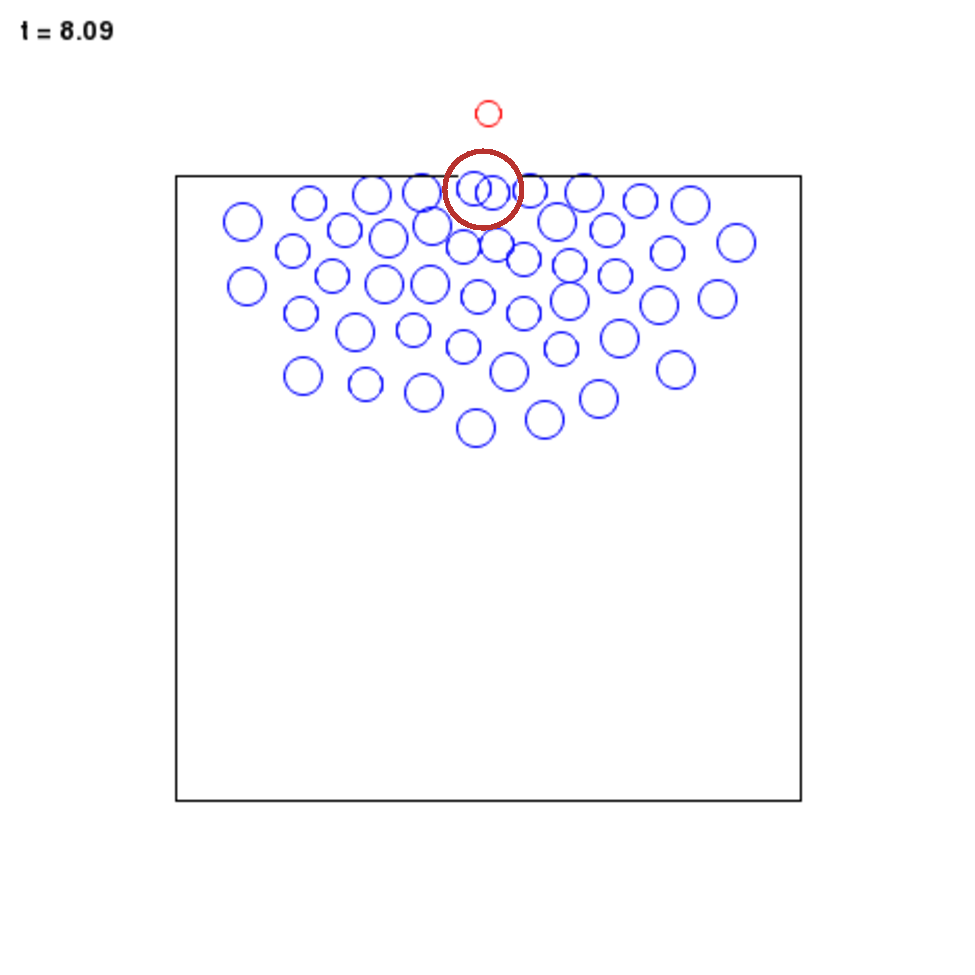
\includegraphics[scale=0.45]{Figures/pedestiranoverlapping.pdf}}
\subfloat[Overlapping between pedestrians and a wall]{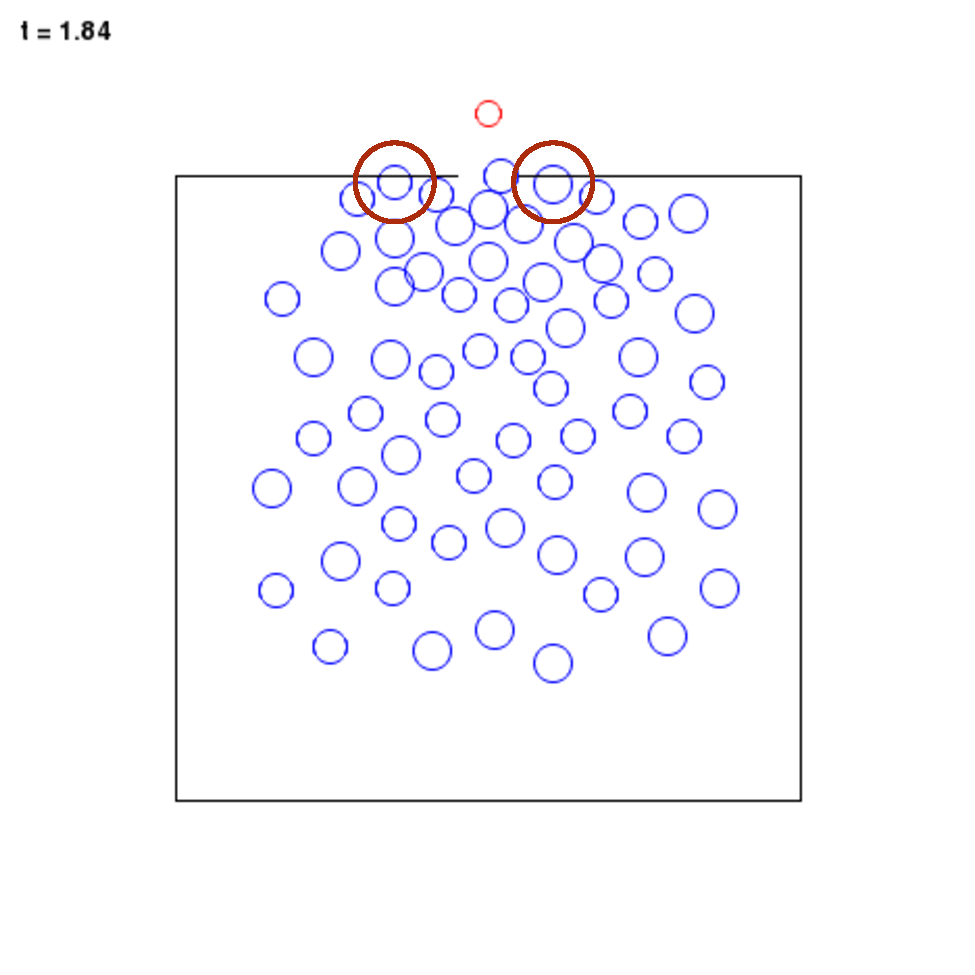
\includegraphics[scale=0.45]{Figures/walloverlapping.pdf}}
\caption{The figure shows two simulations of the squared room. We see the overlapping that can occur between two pedestrians and between the walls and pedestrians. This kind of intersection is seen in most simulations, but they don't cross completely. The red dot on the figures are the desired locations}
\label{fig:overlapping}
\end{figure}

In the figure \ref{fig:overlapping} the overlapping between pedestrians
themselves and between walls and pedestrians. We see that in some situations
it is possible for the pedestrians to intersect quite alot, almost reaching
each others centers. The same thing is seen for the walls, where the wall
can get quite close to the center of a pedestrians. But inspite of this
we don't, with the chosen constants, see that they actually do cross. So
even though it might look like they get sqiuzzed alot together, no completely
unrealistic situations occur. Also we see no other strange scenarios, like
people going in a wrong direction or anything like that. So the most basic
requirements of the model are fulfilled.

We do however see some unrealistic behavior when we change the values in
\ref{tbl:parameter-settings} When looking at some of the different phenomenons,
we need to change certain values like the mean velocity. But when we do
this it starts to get unrealistic. When raising the desired velocity to
a speed like $2.5m/s$, we start to see people crossing each other and going
up to $3.5m/s$ we start to see people crossing the walls. This is a problem
since these results makes no sence to compares with. Lowering the timestep
with $1/10$ doesn't change this result at all. So to solve this problem we
have in some cases raised the wallues of the wall constant $U$ and the
pedestrains repulsion constant $A$. This makes the repulsions forces
big enough for the pedestrians to act 'noraml'. We will throughout the
chapter mention when we change the values and how much it is changed.

\subsection{The phenomena}\label{subsec:ThePhenomena}
In this section we present the results we obtained from our attempts
to replicate the phenomenons presented in \cite{self-org}. These phenomenos are described in section 
\ref{phenomenon}. We will include figure from vairious articles to having something concrete to compare
our results with. The reason we use different articles is because there is not one single article that contains figure of all the scenarios at once. 

\subsubsection{The faster-is-slower effect}
The faster-is-slower was expected to be seen in the square room scenario.
To see if this effects occurs we have looked at the leaving time as a function
of the desired velocity of the pedestrains. We made simulations with a desired
velocitygoing from $1.5m/s$ to $5m/s$ with steps of 0.1. The results are presented
in figure \ref{fig:isfasterslower}. We see some fluctutation on the graph, but the
overall picture of the leaving time decreasing when the desired velocity goes up is
clear. So there no sign of an increase of the leaving time and therefore no faster
is slower. The only thing we see is that the negative slope is decreasing, meaning
that if the pedestrians moves twice as fast, they don't clear the room in half the
time.

\begin{figure}[h]
\centering
\subfloat[Attempt to see the faster-is-slower effect in the square 
room.]{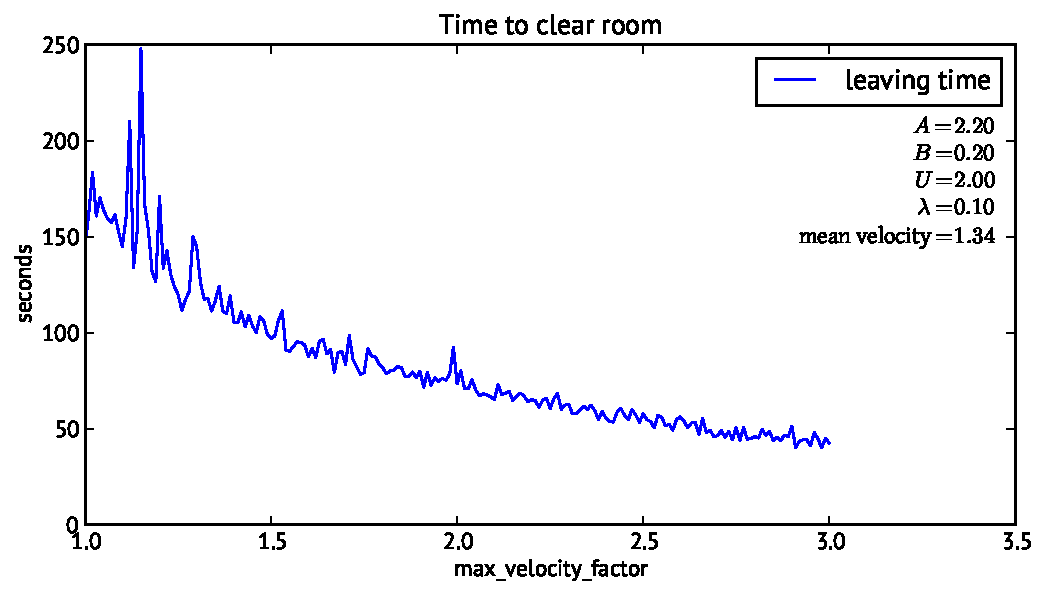
\includegraphics[scale=0.45]{Figures/fastIsSlowNot.pdf}}
\subfloat[Attempt to see the faster-is-slower effect in the normal corridor 
case.]{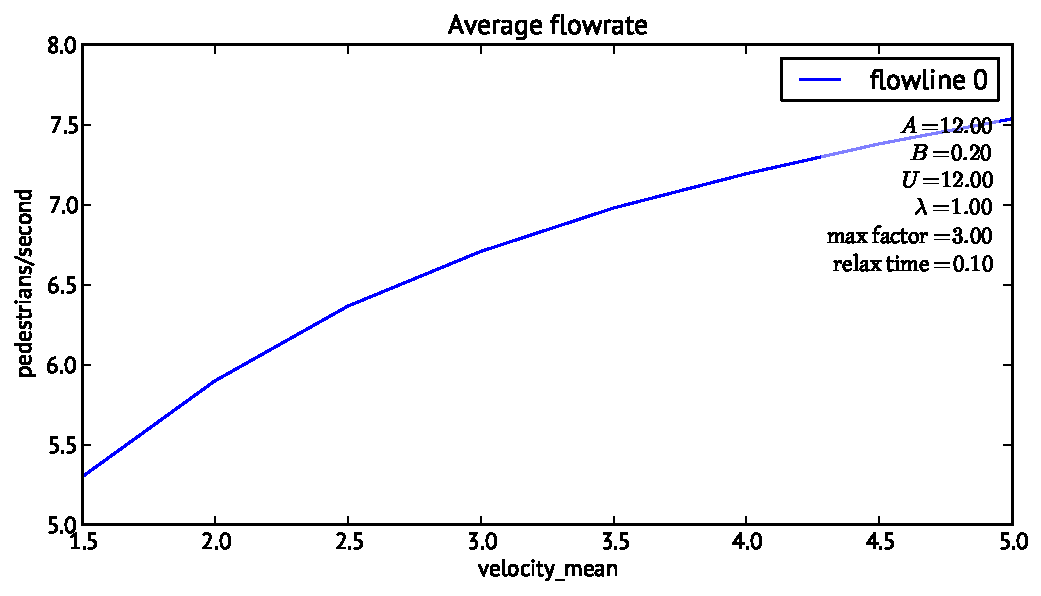
\includegraphics[scale=0.45]{Figures/corridor-flowrate-aggr-velocity_mean.pdf}}\\
\subfloat[Attempt to see the faster-is-slower effect in the bottleneck 
scenario.]{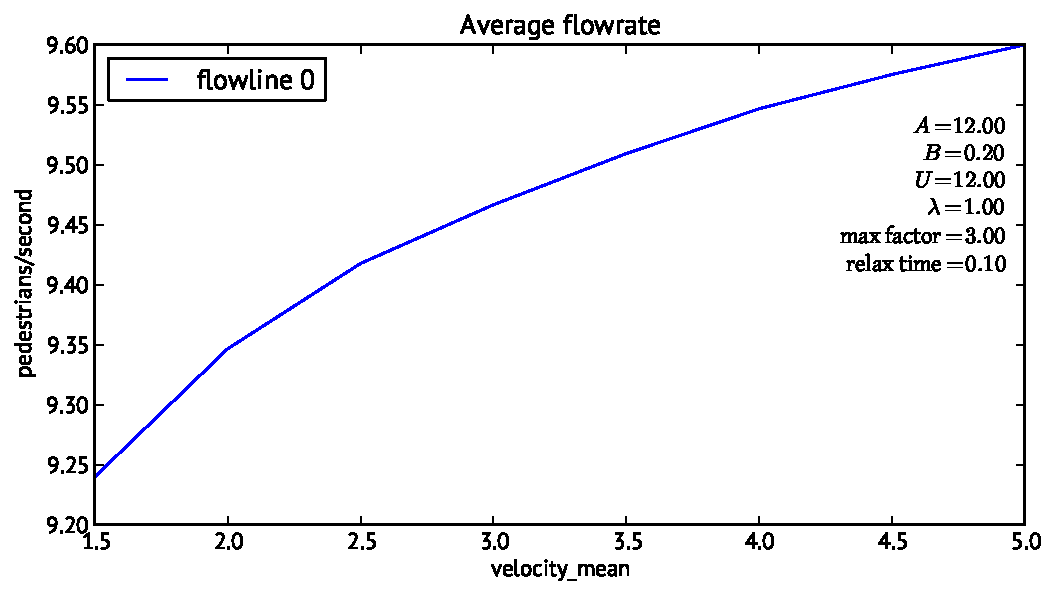
\includegraphics[scale=0.45]{Figures/bottleneck-flowrate-aggr-velocity_mean.pdf}}
\subfloat[Attempt to see the faster-is-slower efffect in the corridor with a 
wide 
space.]{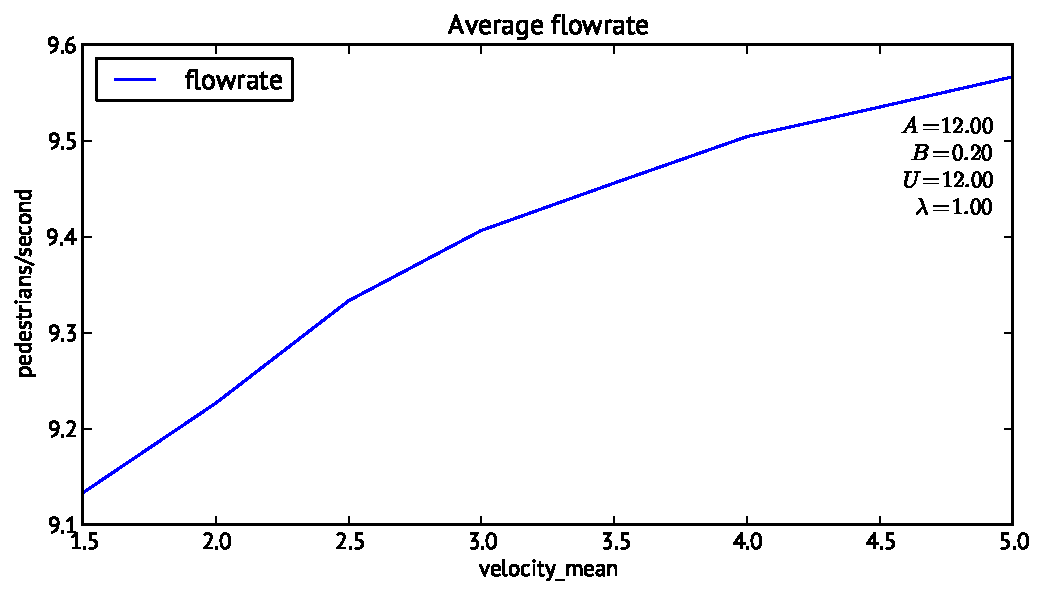
\includegraphics[scale=0.45]{Figures/Wide-kink-one-directional-flowrate-agg.pdf}}
\caption{There is no evidence of the-faster-is slower effect, however it does 
seem that we see a faster-is-only-slightly-faster effect.}
\label{fig:isfasterslower}
\end{figure}
%TODO: We should make runs with the desired velcity.
%This is what they compare with in the letters to nature article.
If we compare with the litterature they show a graph of the leaving time in 
\cite{helbing00}. This graph can be seen on figure 
\ref{fig:LtNFasterIsSlower}. Here it is clearly seen that the leaving time is 
going up when the desired velocity is going up. Quite the opposite result of 
what we are getting. It should be noted that the article these results are 
from, includes tangential forces between the pedestrians. Whereas we do only 
include the repulsion directly away form the pedstrians. In our main article 
\cite{self-org} though, they specific mention the tangential force as making a 
little to none difference in the results. This claim is quoted in section 
\ref{sec:social-forces}.
\begin{figure}[h]
\centering
\subfloat[Square room from case from 
\cite{helbing00}.]{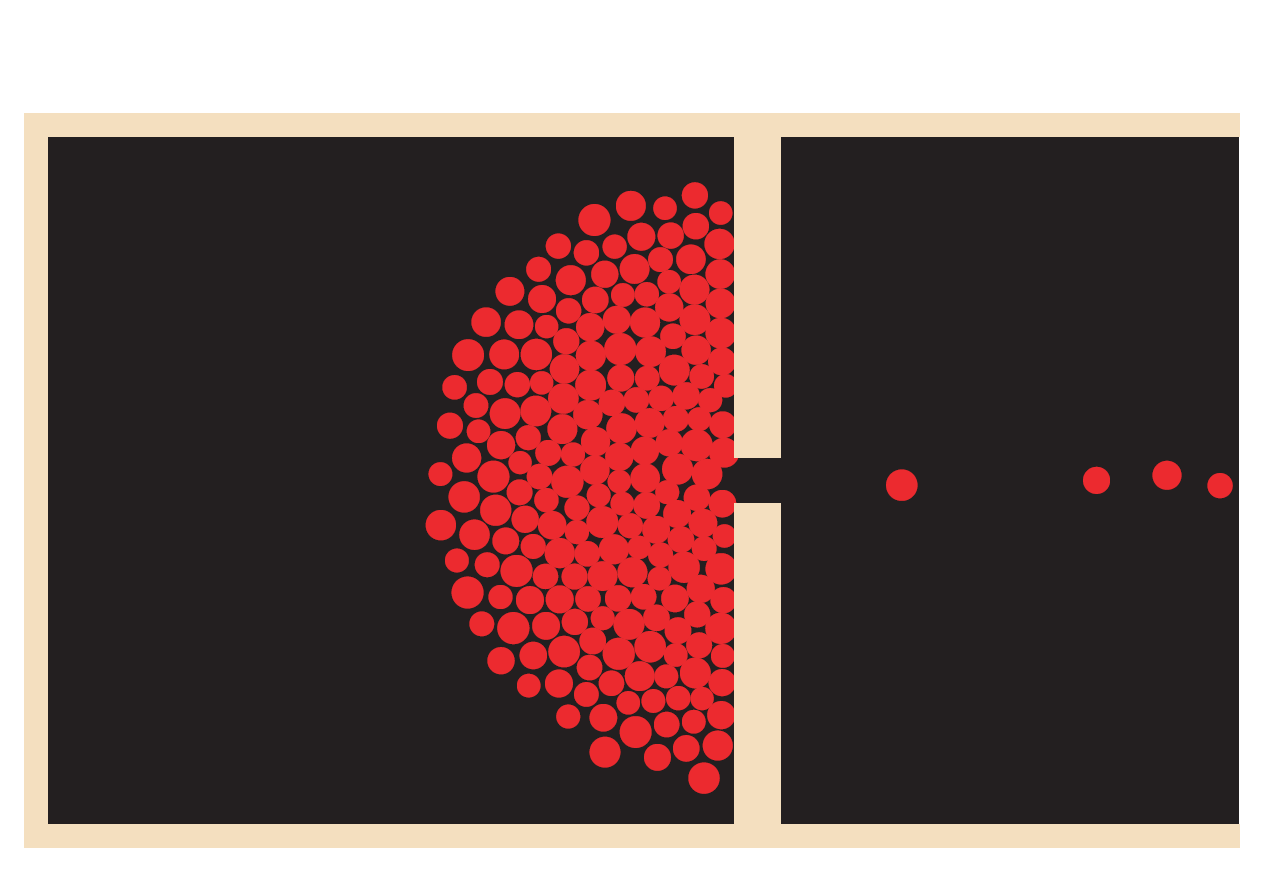
\includegraphics[width=0.45\textwidth]{Figures/square_room_letters.png}}
\subfloat[Graph of the leaving time for the squared room as a function of max. 
desired velocity]{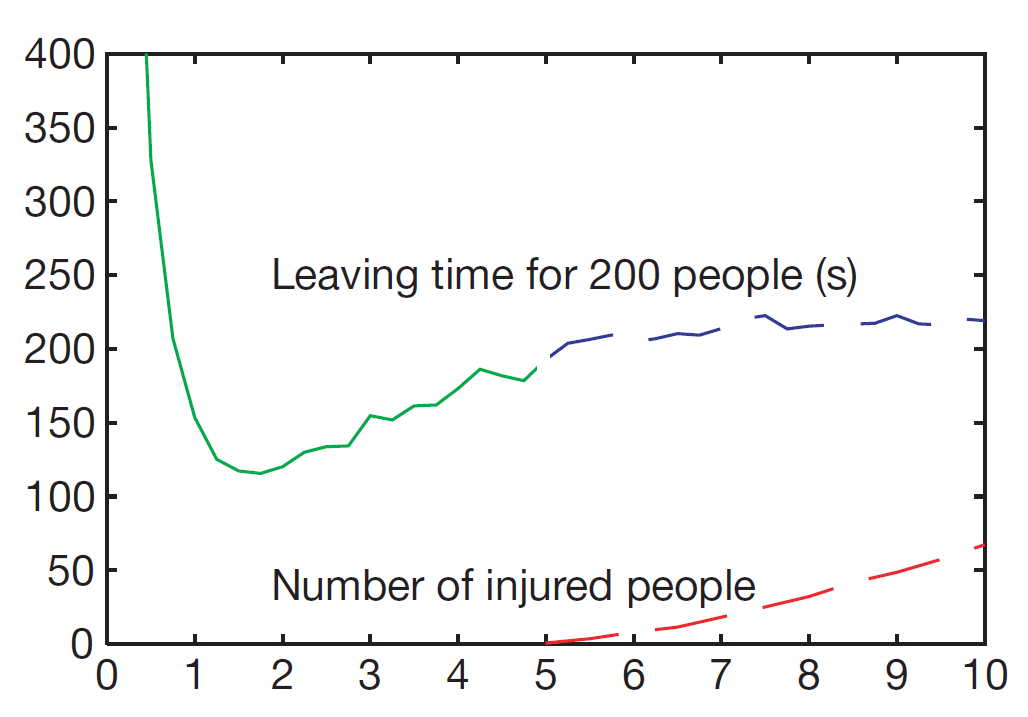
\includegraphics[width=0.45\textwidth]{Figures/leaving_time.png}}
\caption{This is the reuslts for the leaving time as a function of the desired 
velocity. The results are made for a squared romm of $15m*15m$ and $200$ 
pedestrians leaving the room. It is very clear to see that they get the 
faster-is-slower effect.}
\label{fig:LtNFasterIsSlower}
\end{figure}



\subsubsection{Freezing by heating effect}
According to \cite{self-org} the freezing by heating effect should
arise when the max desired velocity of the pedestrians is raised in
situations where there is biderectional flow. We however does not
experience this in any of our simulations of the corridor. We tried
to raise the max velocity, see figure \ref{fig:freezingbyheating1} and
figure \ref{fig:freezingbyheating05}, but instead of observing the
freezing by heating effect, we actually saw that the pedestrians got
through the corridor more easily, and that the density in the corridor
was lower when the max velocity was high. So like the faster is slower
effect again we see no sign of a high desired velocity decreasing/stopping
the movement of the pedestrians.

From the litteratture they show the freezing by heating by showing figures of a complete blocking of the pedestrians. An example of the can be seen on \cite{oscil}, which i shown on figure \ref{fig:freezing_by_heating_litterature}

\begin{figure}[h]
\centering
\subfloat[]{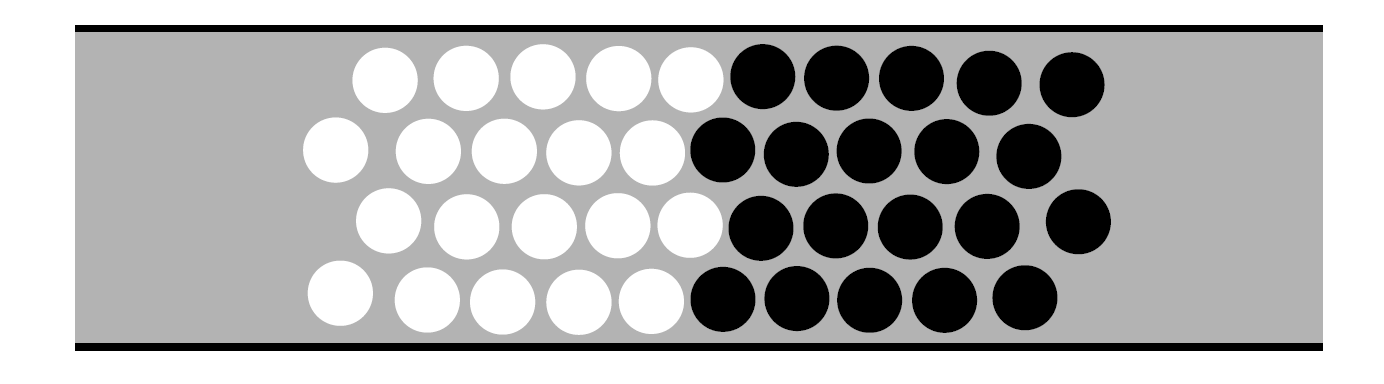
\includegraphics[width=0.45\textwidth]{Figures/heatfreeze.png}}
\caption{Here we can see the pedestrians blocking each other as a result of the freezing by heating. Taken from \cite{oscil}.}
\label{fig:freezing_by_heating_litterature}
\end{figure}


\subsubsection{Lane formation}
Lane formation was expected to happen in the case of bidirectional
flow in corridors. In the article \ref{self-org} you read the following
statement:

\begin{quote}
If pedestrians crowds moving in opposite directions meet each other,
they form small \emph{channels} in the beginning, but these channels
later merge to produce wide lanes
\end{quote}

Since we have three different corridor cases we have looked for lane
formation in all of them. The results are presented in figurewhereas
\ref{fig:laneformation}. Lane formation is observed in every case
and they are of the nature described in \cite{self-org}.\\

\begin{figure}[h]
\centering
\subfloat[]{\resizebox{8cm}{!}{\begin{tikzpicture}
\draw[color=blue] (-2.64,-1.02) circle (0.34);
\draw[color=blue] (-2.89,0.96) circle (0.31);
\draw[color=green] (5.10,-0.19) circle (0.32);
\draw[color=green] (2.19,0.17) circle (0.34);
\draw[color=green] (7.16,-1.49) circle (0.34);
\draw[color=green] (4.10,0.13) circle (0.28);
\draw[color=blue] (-5.87,0.58) circle (0.32);
\draw[color=green] (4.72,-1.57) circle (0.30);
\draw[color=blue] (-0.53,1.69) circle (0.30);
\draw[color=blue] (-2.13,1.68) circle (0.31);
\draw[color=blue] (-5.04,-0.15) circle (0.30);
\draw[color=green] (5.64,-1.69) circle (0.33);
\draw[color=green] (3.38,-1.57) circle (0.32);
\draw[color=blue] (-10.87,-1.75) circle (0.30);
\draw[color=green] (6.43,-0.42) circle (0.31);
\draw[color=green] (2.34,-1.60) circle (0.31);
\draw[color=blue] (-4.76,1.74) circle (0.33);
\draw[color=blue] (-8.66,1.76) circle (0.30);
\draw[color=blue] (-9.81,1.46) circle (0.31);
\draw[color=blue] (-3.52,1.75) circle (0.28);
\draw[color=blue] (-1.27,1.16) circle (0.25);
\draw[color=blue] (-2.06,0.63) circle (0.31);
\draw[color=green] (7.84,-1.70) circle (0.32);
\draw[color=blue] (-1.27,-0.56) circle (0.29);
\draw[color=blue] (-0.27,-0.60) circle (0.35);
\draw[color=green] (1.33,-1.66) circle (0.27);
\draw[color=green] (0.99,0.39) circle (0.30);
\draw[color=blue] (1.08,-0.61) circle (0.30);
\draw[color=blue] (-4.23,-0.62) circle (0.33);
\draw[color=blue] (-6.83,1.76) circle (0.33);
\draw[color=blue] (2.23,1.76) circle (0.29);
\draw[color=blue] (0.34,1.27) circle (0.28);
\draw[color=blue] (1.12,1.73) circle (0.30);
\draw[color=green] (-1.39,-0.16) circle (0.27);
\draw[color=green] (0.26,-1.60) circle (0.28);
\draw[color=green] (-3.13,0.14) circle (0.31);
\draw[color=blue] (5.12,-0.87) circle (0.32);
\draw[color=blue] (2.68,-0.64) circle (0.31);
\draw[color=blue] (4.72,1.61) circle (0.28);
\draw[color=green] (-0.92,-1.72) circle (0.29);
\draw[color=blue] (1.78,0.88) circle (0.28);
\draw[color=blue] (3.41,1.80) circle (0.31);
\draw[color=blue] (3.57,1.05) circle (0.33);
\draw[color=green] (-3.73,0.67) circle (0.32);
\draw[color=green] (-3.21,-1.68) circle (0.28);
\draw[color=green] (-4.56,-1.74) circle (0.29);
\draw[color=green] (-2.18,-1.73) circle (0.30);
\draw[color=green] (-6.02,-0.90) circle (0.31);
\draw[color=green] (-5.41,-0.54) circle (0.30);
\draw[color=blue] (8.22,-1.63) circle (0.30);
\draw[color=blue] (6.29,1.33) circle (0.34);
\draw[color=blue] (5.78,0.55) circle (0.27);
\draw[color=green] (-6.35,0.65) circle (0.28);
\draw[color=green] (-9.00,-1.11) circle (0.29);
\draw[color=blue] (6.83,-0.45) circle (0.34);
\draw[color=green] (-7.61,0.21) circle (0.34);
\draw[color=blue] (7.83,0.76) circle (0.28);
\draw[color=green] (-7.85,-1.11) circle (0.29);
\draw[color=green] (-9.23,0.34) circle (0.32);
\draw[color=green] (-8.66,-0.31) circle (0.31);
%\node at (-12.50, 5.83) {t = 10.12};
\useasboundingbox (-12.50, -5.83) rectangle (12.50, 5.83);
\draw[color=black] (-10.00,2.50) -- (10.00,2.50);
\draw[color=black] (-10.00,-2.50) -- (10.00,-2.50);
\end{tikzpicture}
}}
\subfloat[]{\resizebox{8cm}{!}{\begin{tikzpicture}
\draw[color=blue] (-2.64,-1.02) circle (0.34);
\draw[color=blue] (-2.89,0.96) circle (0.31);
\draw[color=green] (5.10,-0.19) circle (0.32);
\draw[color=green] (2.19,0.17) circle (0.34);
\draw[color=green] (7.16,-1.49) circle (0.34);
\draw[color=green] (4.10,0.13) circle (0.28);
\draw[color=blue] (-5.87,0.58) circle (0.32);
\draw[color=green] (4.72,-1.57) circle (0.30);
\draw[color=blue] (-0.53,1.69) circle (0.30);
\draw[color=blue] (-2.13,1.68) circle (0.31);
\draw[color=blue] (-5.04,-0.15) circle (0.30);
\draw[color=green] (5.64,-1.69) circle (0.33);
\draw[color=green] (3.38,-1.57) circle (0.32);
\draw[color=blue] (-10.87,-1.75) circle (0.30);
\draw[color=green] (6.43,-0.42) circle (0.31);
\draw[color=green] (2.34,-1.60) circle (0.31);
\draw[color=blue] (-4.76,1.74) circle (0.33);
\draw[color=blue] (-8.66,1.76) circle (0.30);
\draw[color=blue] (-9.81,1.46) circle (0.31);
\draw[color=blue] (-3.52,1.75) circle (0.28);
\draw[color=blue] (-1.27,1.16) circle (0.25);
\draw[color=blue] (-2.06,0.63) circle (0.31);
\draw[color=green] (7.84,-1.70) circle (0.32);
\draw[color=blue] (-1.27,-0.56) circle (0.29);
\draw[color=blue] (-0.27,-0.60) circle (0.35);
\draw[color=green] (1.33,-1.66) circle (0.27);
\draw[color=green] (0.99,0.39) circle (0.30);
\draw[color=blue] (1.08,-0.61) circle (0.30);
\draw[color=blue] (-4.23,-0.62) circle (0.33);
\draw[color=blue] (-6.83,1.76) circle (0.33);
\draw[color=blue] (2.23,1.76) circle (0.29);
\draw[color=blue] (0.34,1.27) circle (0.28);
\draw[color=blue] (1.12,1.73) circle (0.30);
\draw[color=green] (-1.39,-0.16) circle (0.27);
\draw[color=green] (0.26,-1.60) circle (0.28);
\draw[color=green] (-3.13,0.14) circle (0.31);
\draw[color=blue] (5.12,-0.87) circle (0.32);
\draw[color=blue] (2.68,-0.64) circle (0.31);
\draw[color=blue] (4.72,1.61) circle (0.28);
\draw[color=green] (-0.92,-1.72) circle (0.29);
\draw[color=blue] (1.78,0.88) circle (0.28);
\draw[color=blue] (3.41,1.80) circle (0.31);
\draw[color=blue] (3.57,1.05) circle (0.33);
\draw[color=green] (-3.73,0.67) circle (0.32);
\draw[color=green] (-3.21,-1.68) circle (0.28);
\draw[color=green] (-4.56,-1.74) circle (0.29);
\draw[color=green] (-2.18,-1.73) circle (0.30);
\draw[color=green] (-6.02,-0.90) circle (0.31);
\draw[color=green] (-5.41,-0.54) circle (0.30);
\draw[color=blue] (8.22,-1.63) circle (0.30);
\draw[color=blue] (6.29,1.33) circle (0.34);
\draw[color=blue] (5.78,0.55) circle (0.27);
\draw[color=green] (-6.35,0.65) circle (0.28);
\draw[color=green] (-9.00,-1.11) circle (0.29);
\draw[color=blue] (6.83,-0.45) circle (0.34);
\draw[color=green] (-7.61,0.21) circle (0.34);
\draw[color=blue] (7.83,0.76) circle (0.28);
\draw[color=green] (-7.85,-1.11) circle (0.29);
\draw[color=green] (-9.23,0.34) circle (0.32);
\draw[color=green] (-8.66,-0.31) circle (0.31);
%\node at (-12.50, 5.83) {t = 10.12};
\useasboundingbox (-12.50, -5.83) rectangle (12.50, 5.83);
\draw[color=black] (-10.00,2.50) -- (10.00,2.50);
\draw[color=black] (-10.00,-2.50) -- (10.00,-2.50);
\end{tikzpicture}
}}\\
\subfloat[]{\resizebox{8cm}{!}{\begin{tikzpicture}
\draw[color=blue] (-2.64,-1.02) circle (0.34);
\draw[color=blue] (-2.89,0.96) circle (0.31);
\draw[color=green] (5.10,-0.19) circle (0.32);
\draw[color=green] (2.19,0.17) circle (0.34);
\draw[color=green] (7.16,-1.49) circle (0.34);
\draw[color=green] (4.10,0.13) circle (0.28);
\draw[color=blue] (-5.87,0.58) circle (0.32);
\draw[color=green] (4.72,-1.57) circle (0.30);
\draw[color=blue] (-0.53,1.69) circle (0.30);
\draw[color=blue] (-2.13,1.68) circle (0.31);
\draw[color=blue] (-5.04,-0.15) circle (0.30);
\draw[color=green] (5.64,-1.69) circle (0.33);
\draw[color=green] (3.38,-1.57) circle (0.32);
\draw[color=blue] (-10.87,-1.75) circle (0.30);
\draw[color=green] (6.43,-0.42) circle (0.31);
\draw[color=green] (2.34,-1.60) circle (0.31);
\draw[color=blue] (-4.76,1.74) circle (0.33);
\draw[color=blue] (-8.66,1.76) circle (0.30);
\draw[color=blue] (-9.81,1.46) circle (0.31);
\draw[color=blue] (-3.52,1.75) circle (0.28);
\draw[color=blue] (-1.27,1.16) circle (0.25);
\draw[color=blue] (-2.06,0.63) circle (0.31);
\draw[color=green] (7.84,-1.70) circle (0.32);
\draw[color=blue] (-1.27,-0.56) circle (0.29);
\draw[color=blue] (-0.27,-0.60) circle (0.35);
\draw[color=green] (1.33,-1.66) circle (0.27);
\draw[color=green] (0.99,0.39) circle (0.30);
\draw[color=blue] (1.08,-0.61) circle (0.30);
\draw[color=blue] (-4.23,-0.62) circle (0.33);
\draw[color=blue] (-6.83,1.76) circle (0.33);
\draw[color=blue] (2.23,1.76) circle (0.29);
\draw[color=blue] (0.34,1.27) circle (0.28);
\draw[color=blue] (1.12,1.73) circle (0.30);
\draw[color=green] (-1.39,-0.16) circle (0.27);
\draw[color=green] (0.26,-1.60) circle (0.28);
\draw[color=green] (-3.13,0.14) circle (0.31);
\draw[color=blue] (5.12,-0.87) circle (0.32);
\draw[color=blue] (2.68,-0.64) circle (0.31);
\draw[color=blue] (4.72,1.61) circle (0.28);
\draw[color=green] (-0.92,-1.72) circle (0.29);
\draw[color=blue] (1.78,0.88) circle (0.28);
\draw[color=blue] (3.41,1.80) circle (0.31);
\draw[color=blue] (3.57,1.05) circle (0.33);
\draw[color=green] (-3.73,0.67) circle (0.32);
\draw[color=green] (-3.21,-1.68) circle (0.28);
\draw[color=green] (-4.56,-1.74) circle (0.29);
\draw[color=green] (-2.18,-1.73) circle (0.30);
\draw[color=green] (-6.02,-0.90) circle (0.31);
\draw[color=green] (-5.41,-0.54) circle (0.30);
\draw[color=blue] (8.22,-1.63) circle (0.30);
\draw[color=blue] (6.29,1.33) circle (0.34);
\draw[color=blue] (5.78,0.55) circle (0.27);
\draw[color=green] (-6.35,0.65) circle (0.28);
\draw[color=green] (-9.00,-1.11) circle (0.29);
\draw[color=blue] (6.83,-0.45) circle (0.34);
\draw[color=green] (-7.61,0.21) circle (0.34);
\draw[color=blue] (7.83,0.76) circle (0.28);
\draw[color=green] (-7.85,-1.11) circle (0.29);
\draw[color=green] (-9.23,0.34) circle (0.32);
\draw[color=green] (-8.66,-0.31) circle (0.31);
%\node at (-12.50, 5.83) {t = 10.12};
\useasboundingbox (-12.50, -5.83) rectangle (12.50, 5.83);
\draw[color=black] (-10.00,2.50) -- (10.00,2.50);
\draw[color=black] (-10.00,-2.50) -- (10.00,-2.50);
\end{tikzpicture}
}}
\caption{Lane formation in the different corridors.}
\label{fig:laneformation}
\end{figure}

From the litterature we can see that they present figures of lane formations
 that looks like what we are seeing. They do how ever manily stick with the normal corridor. One of these results are shown in \cite{lanes}, which can be seen on figure \ref{fig:laneformation_litterature}
\begin{figure}[h]
\centering
\subfloat[]{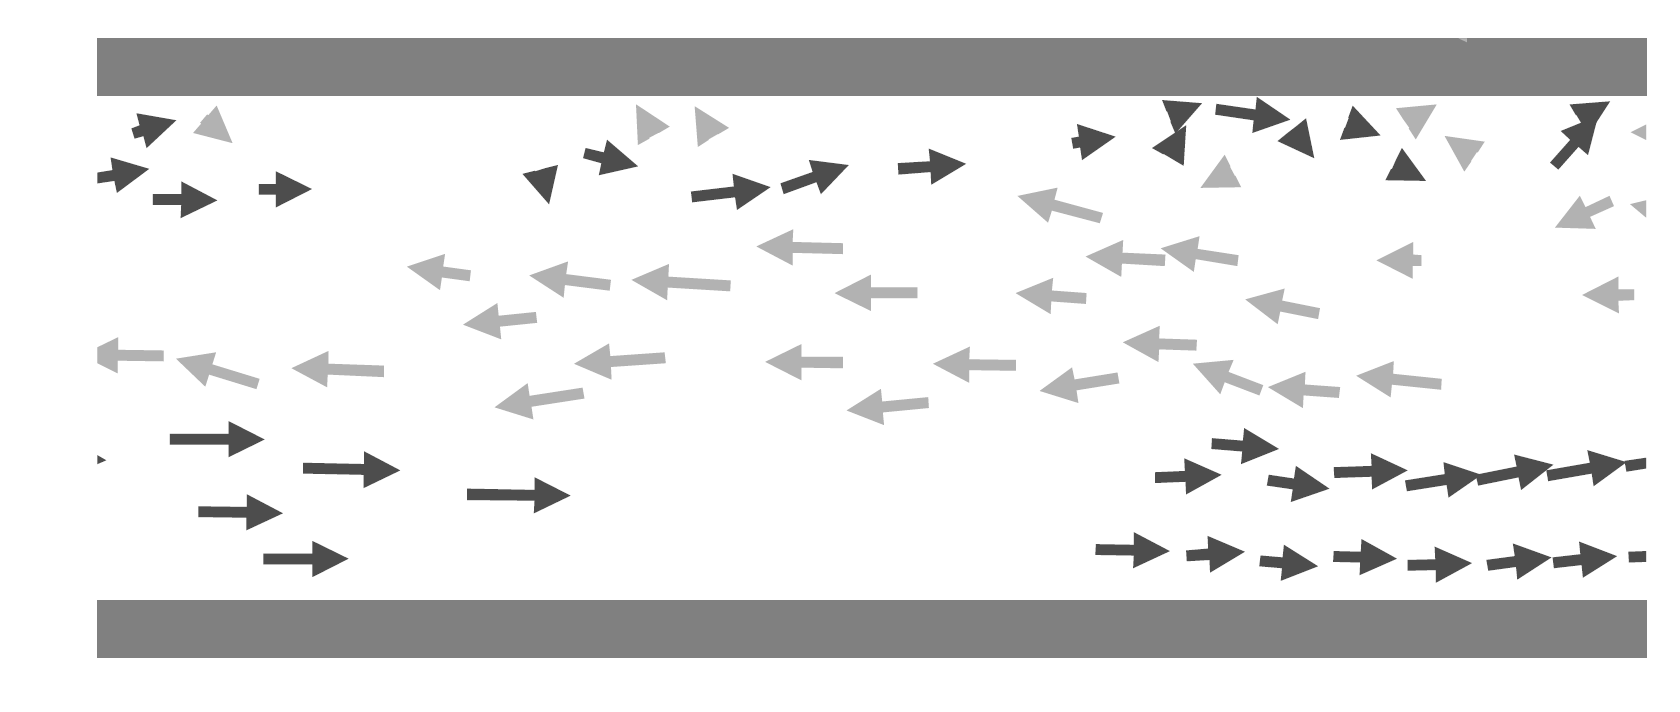
\includegraphics[width=8cm]{Figures/flow_lanes_litterature.png}}
\caption{Lane formation through a corridor. Taken from \cite{lanes}.}
\label{fig:laneformation_litterature}
\end{figure}
 


\subsubsection{The Oscillatory flow}
The oscillatory flow is expected to arise in the case of bidirectional
flow through a bottleneck. The results are presented in figure
\ref{fig:oscillitoryflow}.\\

\begin{figure}[h]
\centering
{\resizebox{7cm}{!}{\begin{tikzpicture}
\draw[color=blue] (-2.64,-1.02) circle (0.34);
\draw[color=blue] (-2.89,0.96) circle (0.31);
\draw[color=green] (5.10,-0.19) circle (0.32);
\draw[color=green] (2.19,0.17) circle (0.34);
\draw[color=green] (7.16,-1.49) circle (0.34);
\draw[color=green] (4.10,0.13) circle (0.28);
\draw[color=blue] (-5.87,0.58) circle (0.32);
\draw[color=green] (4.72,-1.57) circle (0.30);
\draw[color=blue] (-0.53,1.69) circle (0.30);
\draw[color=blue] (-2.13,1.68) circle (0.31);
\draw[color=blue] (-5.04,-0.15) circle (0.30);
\draw[color=green] (5.64,-1.69) circle (0.33);
\draw[color=green] (3.38,-1.57) circle (0.32);
\draw[color=blue] (-10.87,-1.75) circle (0.30);
\draw[color=green] (6.43,-0.42) circle (0.31);
\draw[color=green] (2.34,-1.60) circle (0.31);
\draw[color=blue] (-4.76,1.74) circle (0.33);
\draw[color=blue] (-8.66,1.76) circle (0.30);
\draw[color=blue] (-9.81,1.46) circle (0.31);
\draw[color=blue] (-3.52,1.75) circle (0.28);
\draw[color=blue] (-1.27,1.16) circle (0.25);
\draw[color=blue] (-2.06,0.63) circle (0.31);
\draw[color=green] (7.84,-1.70) circle (0.32);
\draw[color=blue] (-1.27,-0.56) circle (0.29);
\draw[color=blue] (-0.27,-0.60) circle (0.35);
\draw[color=green] (1.33,-1.66) circle (0.27);
\draw[color=green] (0.99,0.39) circle (0.30);
\draw[color=blue] (1.08,-0.61) circle (0.30);
\draw[color=blue] (-4.23,-0.62) circle (0.33);
\draw[color=blue] (-6.83,1.76) circle (0.33);
\draw[color=blue] (2.23,1.76) circle (0.29);
\draw[color=blue] (0.34,1.27) circle (0.28);
\draw[color=blue] (1.12,1.73) circle (0.30);
\draw[color=green] (-1.39,-0.16) circle (0.27);
\draw[color=green] (0.26,-1.60) circle (0.28);
\draw[color=green] (-3.13,0.14) circle (0.31);
\draw[color=blue] (5.12,-0.87) circle (0.32);
\draw[color=blue] (2.68,-0.64) circle (0.31);
\draw[color=blue] (4.72,1.61) circle (0.28);
\draw[color=green] (-0.92,-1.72) circle (0.29);
\draw[color=blue] (1.78,0.88) circle (0.28);
\draw[color=blue] (3.41,1.80) circle (0.31);
\draw[color=blue] (3.57,1.05) circle (0.33);
\draw[color=green] (-3.73,0.67) circle (0.32);
\draw[color=green] (-3.21,-1.68) circle (0.28);
\draw[color=green] (-4.56,-1.74) circle (0.29);
\draw[color=green] (-2.18,-1.73) circle (0.30);
\draw[color=green] (-6.02,-0.90) circle (0.31);
\draw[color=green] (-5.41,-0.54) circle (0.30);
\draw[color=blue] (8.22,-1.63) circle (0.30);
\draw[color=blue] (6.29,1.33) circle (0.34);
\draw[color=blue] (5.78,0.55) circle (0.27);
\draw[color=green] (-6.35,0.65) circle (0.28);
\draw[color=green] (-9.00,-1.11) circle (0.29);
\draw[color=blue] (6.83,-0.45) circle (0.34);
\draw[color=green] (-7.61,0.21) circle (0.34);
\draw[color=blue] (7.83,0.76) circle (0.28);
\draw[color=green] (-7.85,-1.11) circle (0.29);
\draw[color=green] (-9.23,0.34) circle (0.32);
\draw[color=green] (-8.66,-0.31) circle (0.31);
%\node at (-12.50, 5.83) {t = 10.12};
\useasboundingbox (-12.50, -5.83) rectangle (12.50, 5.83);
\draw[color=black] (-10.00,2.50) -- (10.00,2.50);
\draw[color=black] (-10.00,-2.50) -- (10.00,-2.50);
\end{tikzpicture}
}}
\caption{A screen shot of bidirectional flow in the bottlenck}
\label{fig:oscillitoryflow}
\end{figure}

When looking at the simulation while it is running it is not
immediately clear that the oscillatory flow occurs. Clogging
appears in both ends of the bottleneck and people are sometimes
squeezed through the bottleneck. The graph presented in
\ref{fig:oscillitoryflow} does indicate that the oscillatory
flow occurs.

In the article \cite{oscil}, they show a figure of the oscillatory flow. They 
don't show any graph of the flow in different directions or anything like 
that, but basicly just shows a screen shot giving some idea about the 
phenomena along with a discribtion of the phenomena. They describe it as the 
pressure building up from one side and the at some point a small group of 
pedestrians slip through. When that happens the pressure on the other side 
builds up and then at some time some pedestrians from that side slips through 
and so on. Figure \ref{fig:oscillitoryflow_litterature} shows the 
presentations of the oscillatory flow from \cite{oscil}. This describtions 
fits with what we ourself experince through simulations of the model too.

\begin{figure}[h]
\centering
\subfloat[Screen shot of oscillatory flow from 
\cite{oscil}]{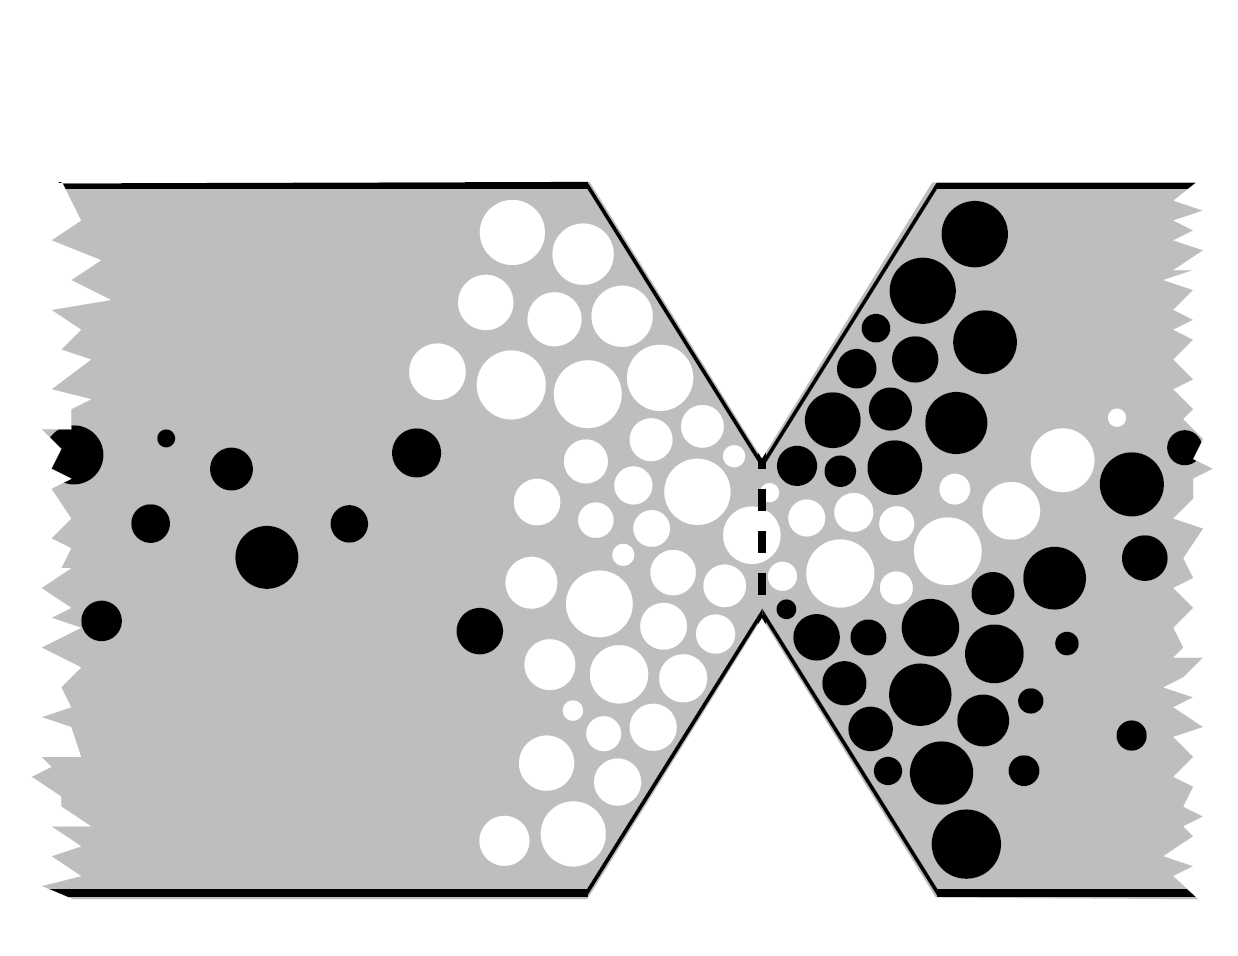
\includegraphics[width=0.5\textwidth]{Figures/oscil_flow.png}}
\caption{Here one can see that some black pedestrians that already have slip through and now the white pedestrians going in the other direction a passing through the bottleneck.}
\label{fig:oscillitoryflow_litterature}
\end{figure}


\subsection{Summery}
We have been able to get a working simulation of the social force model 
presented in \cite{self-org} with components taken from \cite{ABconstant}. 
The most basic dynamics og the simulations seems to be running like as it 
should and our simulations show lane formation in bidirectional flow. We also  
see oscillatory flow at bottlenecks however freezin-by-heating 
and faster-is-slower effect is not observed at all.
